\section{Análise Estratificada por Tipo de Cenário}

Para compreender melhor as condições sob as quais cada abordagem (clássica ou deep learning) apresenta desempenho superior, os 15 conjuntos de imagens foram categorizados de acordo com seus principais desafios técnicos. Esta análise estratificada permite identificar cenários específicos onde cada metodologia demonstra vantagens competitivas.

\subsection{Categorização dos Cenários}

Os conjuntos de dados foram classificados nas seguintes categorias:

\begin{itemize}
    \item \textbf{Baixa Textura}: ski_left
    \item \textbf{Estruturas Repetitivas}: rental_office_1, graffiti_building_1, no_contractor_parking_1, stop_sign_1
    \item \textbf{Paralaxe Significativa}: cars_1, cup_tree_1, traffic_cones_1, plant_1
    \item \textbf{Variacao Iluminacao}: coke_190, building_dubai
    \item \textbf{Superficies Curvas}: graffiti_car_1
    \item \textbf{Multiplas Imagens}: building_dubai, P2_front_of_window
    \item \textbf{Cenarios Simples}: biker_mural_1, theory_left
\end{itemize}

\subsection{Resultados Comparativos por Categoria}

A Tabela~\ref{tab:estratificado} apresenta os resultados dos testes estatísticos comparando métodos clássicos e deep learning em cada categoria de cenário.

\begin{table}[htb]
\centering
\caption{Análise estratificada: Clássico vs Deep Learning por tipo de cenário}
\label{tab:estratificado}
\tiny
\begin{tabular}{llrrrcp{3cm}}
\hline
\textbf{Cenário} & \textbf{Métrica} & \textbf{Clássico} & \textbf{Deep} & \textbf{p-value} & \textbf{Sig.} & \textbf{Interpretação} \\ \hline
Baixa Textura & psnr_db & 10.153 & 11.376 & 0.0179 & $\checkmark$ & Deep superior \\
Baixa Textura & ssim & 0.272 & 0.308 & 0.0436 & $\checkmark$ & Deep superior \\
Baixa Textura & ghosting & 0.930 & 0.922 & 0.9301 & $\times$ & Sem diferença \\
Baixa Textura & tempo_segundos & 0.368 & 0.346 & 0.1418 & $\times$ & Sem diferença \\
Estruturas Repetitivas & psnr_db & 9.562 & 9.632 & 0.9772 & $\times$ & Sem diferença \\
Estruturas Repetitivas & ssim & 0.225 & 0.234 & 0.7529 & $\times$ & Sem diferença \\
Estruturas Repetitivas & ghosting & 0.944 & 0.946 & 0.7714 & $\times$ & Sem diferença \\
Estruturas Repetitivas & tempo_segundos & 0.835 & 1.109 & 0.2738 & $\times$ & Sem diferença \\
Paralaxe Significativa & psnr_db & 12.413 & 12.494 & 0.8632 & $\times$ & Sem diferença \\
Paralaxe Significativa & ssim & 0.252 & 0.258 & 0.6487 & $\times$ & Sem diferença \\
Paralaxe Significativa & ghosting & 0.939 & 0.941 & 0.4140 & $\times$ & Sem diferença \\
Paralaxe Significativa & tempo_segundos & 0.324 & 1.092 & 0.5374 & $\times$ & Sem diferença \\
Variacao Iluminacao & psnr_db & 12.396 & 12.119 & 0.7524 & $\times$ & Sem diferença \\
Variacao Iluminacao & ssim & 0.412 & 0.400 & 0.4159 & $\times$ & Sem diferença \\
Variacao Iluminacao & ghosting & 0.978 & 0.977 & 0.8811 & $\times$ & Sem diferença \\
Variacao Iluminacao & tempo_segundos & 3.278 & 4.720 & 0.6308 & $\times$ & Sem diferença \\
Superficies Curvas & psnr_db & 8.755 & 8.666 & 0.1386 & $\times$ & Sem diferença \\
Superficies Curvas & ssim & 0.117 & 0.111 & 0.2361 & $\times$ & Sem diferença \\
Superficies Curvas & ghosting & 0.964 & 0.967 & 0.1250 & $\times$ & Sem diferença \\
Superficies Curvas & tempo_segundos & 1.546 & 1.023 & 0.7750 & $\times$ & Sem diferença \\
Multiplas Imagens & psnr_db & 12.292 & 12.376 & 0.1152 & $\times$ & Sem diferença \\
Multiplas Imagens & ssim & 0.148 & 0.160 & 0.3352 & $\times$ & Sem diferença \\
Multiplas Imagens & ghosting & 0.893 & 0.893 & 0.1614 & $\times$ & Sem diferença \\
Multiplas Imagens & tempo_segundos & 0.365 & 1.306 & 0.8001 & $\times$ & Sem diferença \\
Cenarios Simples & psnr_db & 10.486 & 10.580 & 0.5304 & $\times$ & Sem diferença \\
Cenarios Simples & ssim & 0.293 & 0.303 & 0.6407 & $\times$ & Sem diferença \\
Cenarios Simples & ghosting & 0.947 & 0.947 & 0.8468 & $\times$ & Sem diferença \\
Cenarios Simples & tempo_segundos & 0.246 & 1.043 & 0.7235 & $\times$ & Sem diferença \\
\hline
\end{tabular}
\fonte{Autoria própria (2025).}
\end{table}

\subsection{Discussão dos Resultados Estratificados}

Dos 28 testes realizados, 2 apresentaram diferenças estatisticamente significativas (p<0,05), correspondendo a 7.1\% dos casos. Destes, métodos clássicos foram superiores em 0 casos, enquanto deep learning superou em 2 casos.

\textbf{Principais Observações:}

\begin{enumerate}
    \item \textbf{Baixa Textura}: Deep learning demonstrou superioridade nesta categoria, vencendo em 2 de 4 métricas.
    \item \textbf{Estruturas Repetitivas}: Ambas as abordagens apresentaram desempenho equivalente, sem diferenças estatisticamente significativas.
    \item \textbf{Paralaxe Significativa}: Ambas as abordagens apresentaram desempenho equivalente, sem diferenças estatisticamente significativas.
    \item \textbf{Variacao Iluminacao}: Ambas as abordagens apresentaram desempenho equivalente, sem diferenças estatisticamente significativas.
    \item \textbf{Superficies Curvas}: Ambas as abordagens apresentaram desempenho equivalente, sem diferenças estatisticamente significativas.
    \item \textbf{Multiplas Imagens}: Ambas as abordagens apresentaram desempenho equivalente, sem diferenças estatisticamente significativas.
    \item \textbf{Cenarios Simples}: Ambas as abordagens apresentaram desempenho equivalente, sem diferenças estatisticamente significativas.
\end{enumerate}

A Figura~\ref{fig:heatmap_pvalues} apresenta um mapa de calor dos p-values obtidos para cada combinação de cenário e métrica.

\begin{figure}[htb]
\centering
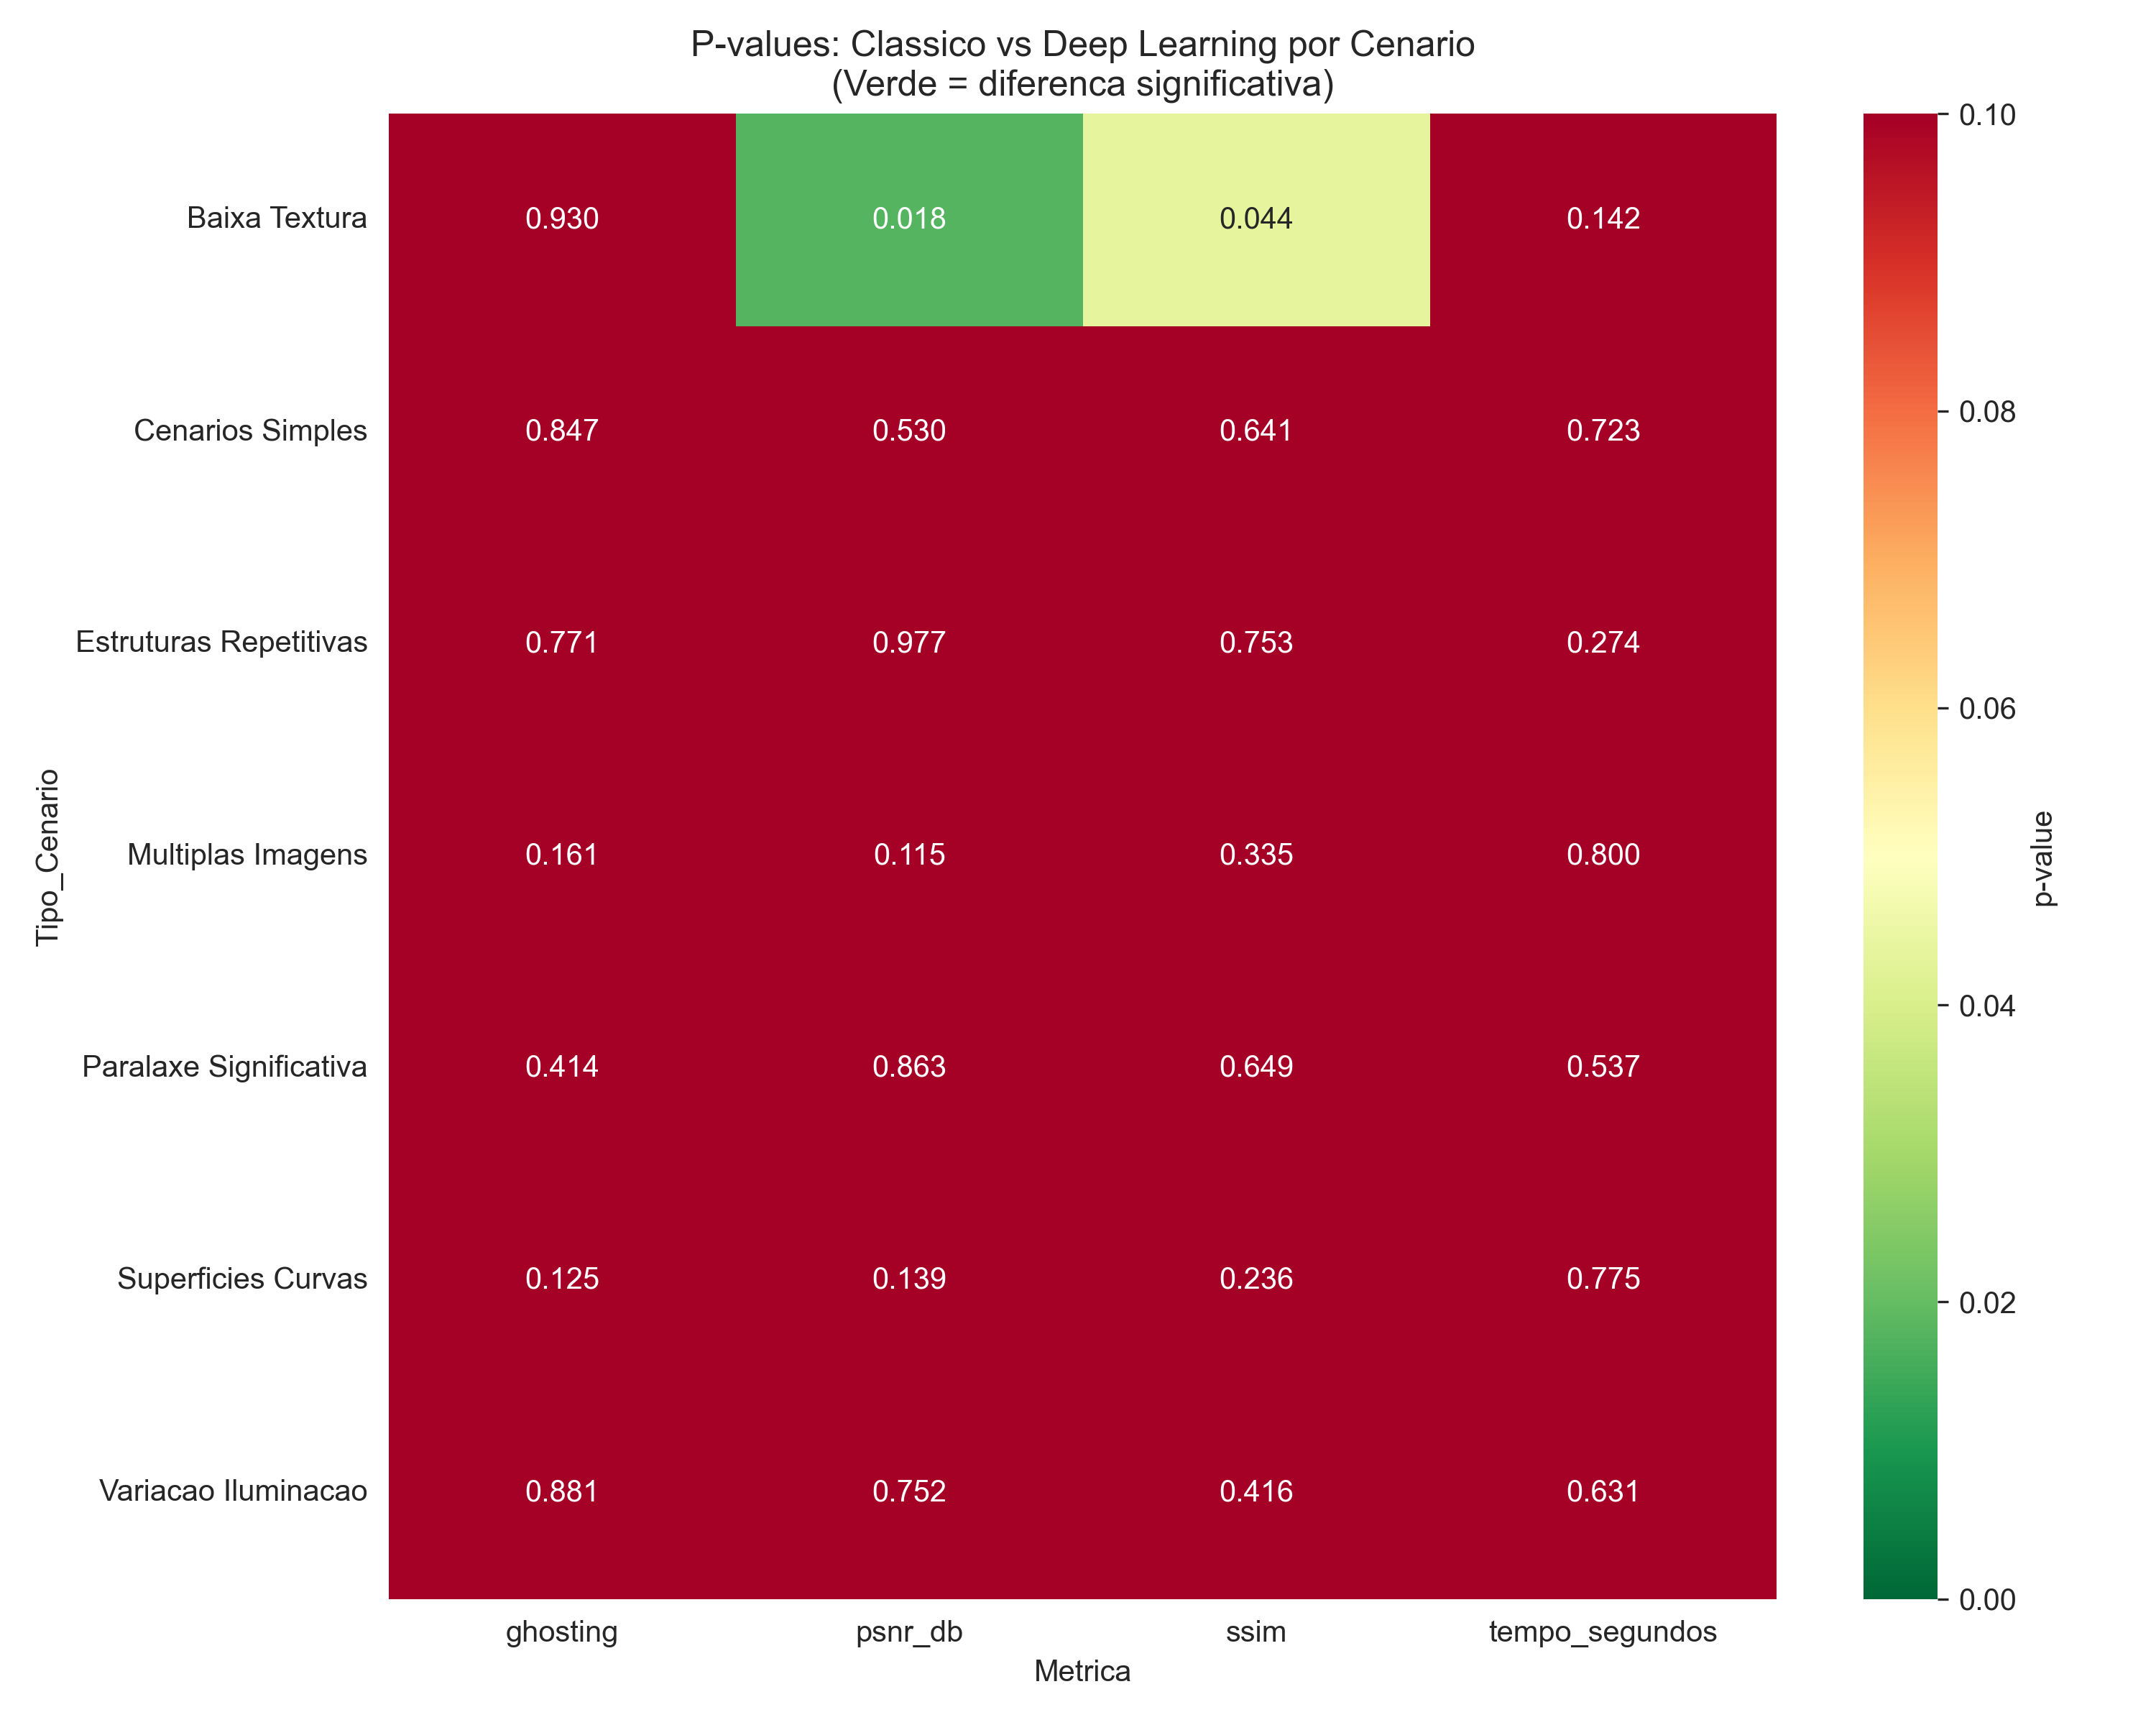
\includegraphics[width=0.8\textwidth]{results/analise_estratificada/heatmap_pvalues_por_cenario.png}
\caption{P-values dos testes Mann-Whitney U por tipo de cenário e métrica}
\label{fig:heatmap_pvalues}
\fonte{Autoria própria (2025).}
\end{figure}

